\chapter{Introduction}\label{chap:intro}

Understanding the physical processes which shaped our Universe is the fundamental goal of all fields in astrophysics. A theory of the Universe must describe how it evolved from the primordial soup of matter present just after the Big Bang to the whole host of galaxy properties we see today. 

At the time of writing, the most widely accepted model is the $\Lambda-\rm{CDM}$ ($\Lambda-$ cold dark matter) model which describes a flat Universe made of only $\sim4\%$ baryonic (``normal'') matter, $\sim21\%$ cold dark matter and $\sim71\%$ dark energy \citep{planck16}. In such a Universe, tiny quantum fluctuations in the early Universe grow with time, becoming overdense and lay the foundations for galaxy formation. Given the very small fraction of baryonic matter in the Universe, its gravitational contribution to this process is often neglected, greatly simplifying the problem. Structure is then observed to form hierarchically in simulations \citep{citebomb}. At the overdense regions in the early Universe, matter collapses dissipationally under its own gravity forming a dark matter `halo', which then grows through smooth accretion and mergers of other halos to produce objects with the wide range of masses we observe in the Universe today. 

Adding in the complex baryonic physics into this picture however, complicates matters. Galaxies are, unfortunately, not just simple smooth dark matter halos; they are thought to start life when baryons cool and condense at the centre of a dark matter halo. Further accretion of circum-nuclear gas then forms a rotating disc, within which stars will form as hydrogen gas coalesces and a galaxy is born. From this moment a galaxy will evolve, its shape changing depending on its encounters (or lack thereof) with other galaxies. 

Today we observe galaxies of a multitude of shapes, or morphology, across all redshift ranges. \cite{hubble36}  was the first to classify galaxies based on their shape, producing the widely adopted `tuning fork diagram', now known as the Hubble sequence and shown in Figure~\ref{fig:hubble}. Hubble noticed that galaxies could by broadly categorised as either elliptical in shape or as a disc with spiral arms and barred structures. He referred to these categories as early-types (and put them to the left of his diagram, in keeping with time axis conventions) and late types respectively, as he thought that as galaxies evolved they developed spiral structure. However, as discussed above, cosmological studies have concluded that galaxies start life as a rotating gas disc and so instead Hubble's diagram is often read from right to left. Connecting this picture of pure gas disc galaxies in their infancy, with this plethora of galaxy structure we see today, is the focus of this thesis. 

\begin{figure}
\centering{
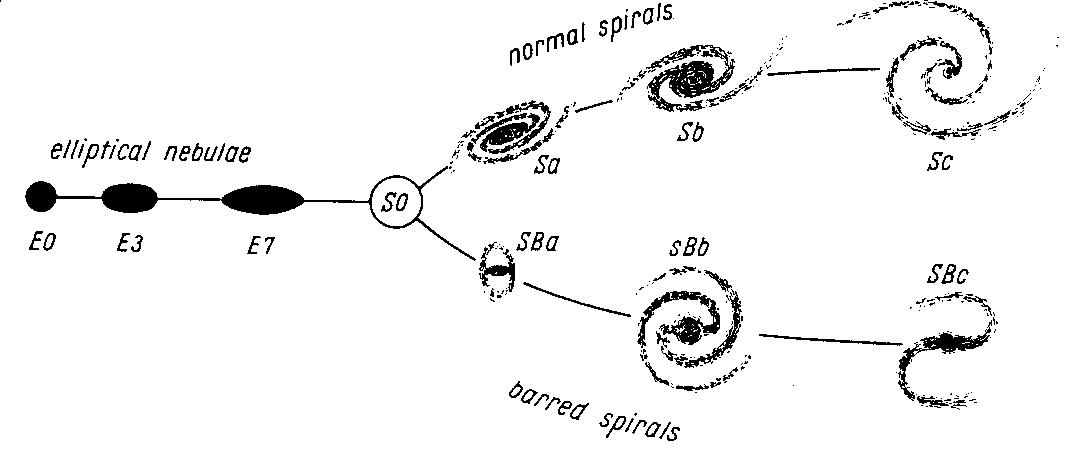
\includegraphics[width=\textwidth]{introduction/hubble.jpeg}}
\caption[The Hubble sequence for morphological classification of galaxies]{The Hubble sequence of galaxy morphology shown on his famous `tuning fork diagram' as published in \cite{hubble36}.}
\label{fig:hubble}
\end{figure}

Like all difficult problems however, the structure alone is not enough to describe a galaxy's evolution. The magnitude (used as a proxy for stellar mass), star formation rate (SFR) and metallicity (Z) are all crucial to describing a galaxy's current state. By studying these galaxy properties, insight into the processes which govern galaxy evolution can be gained.

Large scale surveys of galaxies have revealed a bimodality in the optical colour-magnitude diagram (CMD) finding two distinct populations; one at relatively low mass, with blue optical colours and another at relatively high mass, with red optical colours \citep{Baldry04, Baldry06, Willmer06, ball08, Brammer09}. These populations were dubbed the `blue cloud' and `red sequence' respectively \citep{Chester64, bower92, Driver06, Faber07}.  The sparsely populated colour space between these two populations was dubbed the  `green valley'.

The majority of disc galaxies were found in the blue cloud and the majority of ellipticals on the red sequence, with colour often used as a proxy for morphology. The Galaxy Zoo project \citep{Lintott11}, which produced morphological classifications for a million galaxies, helped to confirm that this colour bimodality is not entirely morphology driven \citep{Strat01, Salim07, Sch07, CHV08, Bamford09, Skibba09}, detecting larger numbers of spiral galaxies in the red sequence \citep{masters10c} and elliptical galaxies in the blue cloud \citep{Sch09} than had previously been detected.

Star forming galaxies are also observed to lie on a well defined `star forming sequence' (SFS) in the stellar mass vs. star formation rate (SFR) plane. The majority of blue cloud galaxies are found to lie on this SFS with the majority of the red sequence lying well below it with very low SFRs. The intermediate colours of the green valley have therefore been interpreted as evidence of recent suppression of star formation \citep[SF;][]{Salim07}. This suppression of SF and subsequent transition of a galaxy from blue cloud to red sequence must therefore also be intrinsically tied with a possible change in morphology from a disc galaxy to an elliptical galaxy.

Green valley galaxies have therefore long been thought of as the `crossroads' of galaxy evolution, a transition population between the two main galactic stages of the star forming blue cloud and the `dead' red sequence \citep{Bell04, Wyder07, Schim07, Martin07, Faber07, Mendez11, Gonc12, schawinski14, Pan14}. This transition is theorised to occur on rapid timescales, otherwise there would be an accumulation of galaxies residing in the green valley, rather than an accumulation in the red sequence as is observed \citep{Arnouts07, Martin07}.

I will refer to this suppression of a galaxy's SFR as \emph{quenching} and processes which can cause this suppression as \emph{quenching mechanisms}. By studying these galaxies which are quenching, having just left the SFS sequence, the mechanisms governing large scale galaxy evolution, including both the suppression of SF and the possible transformation of galaxy structure, can be probed. 

\section{Possible quenching mechanisms}\label{sec:quenchmech}

There are many theorised mechanisms which can cause quenching. They are often referred to as either \emph{internal} mechanisms (caused by the galaxy's \emph{nature}) or \emph{external} mechanisms (caused by the way the galaxy is \emph{nurtured}). The properties of a galaxy and its environment are often thought to control which mechanisms will affect a galaxy throughout its lifetime and subsequently affect the morphology. 

%There have been many previous theories for the initial triggers of these quenching mechanisms, including negative feedback from AGN \citep{diMatteo05, Martin07, Nandra07, Sch07}, mergers \citep{Darg10a, Cheung12, Barro13}, supernovae winds \citep{MFB12}, cluster interactions \citep{Coil08, Mendez11, Fang13} and secular evolution \citep{masters10c, masters11a, Mendez11}. By investigating the \emph{amount} of quenching that has occurred in the blue cloud, green valley and red sequence; and by comparing the amount across these three populations, I can apply some constraints to these theories. 
\subsection{Internal Quenching Mechanisms}\label{sec:intquench}

\subsubsection{AGN feedback as a quenching mechanism}\label{sec:agnquench}

An active galactic nucleus (AGN) is an actively growing super massive black hole in the central of a galaxy. During accretion of material onto an AGN, it can output energetic material which can either heat or expel gas needed for SF in a galaxy, causing quenching. AGN feedback was first suggested as a mechanism for regulating star formation due to the results of simulations \citep{silk98, Croton06, Bower06, somerville08} wherein galaxies grew to unrealistic stellar masses. Without a prescription for the effects of AGN feedback, the shape of the galaxy luminosity function \citep{} could not be matched at the high luminosity end (a similar problem was encountered at the low end of the luminosity function, which was rectified by the inclusion of the effects of supernova wind feedback; \citealt{}). AGN feedback is one of the most studied mechanisms of quenching due to the nature of the observed co-evolution of galaxies and their central supermassive black holes \citep{magorrian98, marconi03, haringrix04}. 

Indirect observational evidence has now ben found for both positive and negative feedback in various systems (see the comprehensive review from \citealt{fabian12}). The strongest of which is that the largest fraction of AGN are found in the green valley \citep{cowie08, Hickox09, schawinski10a}, suggesting some link between AGN activity and the process which moves a galaxy from the blue cloud to the red sequence. However, concrete statistical evidence for the effect of AGN feedback on the host galaxy population has so far been elusive.

%There are many mechanisms which are proposed to cause quenching; including mergers \citep{daddi10, darg10b, cheung12, barro13, pontzen16}, AGN feedback \citep{dimatteo05, nandra07}, mass quenching \citep{peng12}, morphological quenching \citep{fang13} and the environment of a galaxy \citep[see review of mechanisms in][and references therein]{boselli06}.

\subsubsection{Mass quenching}\label{sec:massquench}
Mass quenching is the process by which a galaxy, independent of its environment, uses up its available gas for star formation via the Kennicutt-Schmidt law \citep{schmidt59, kennicutt98} and consequently grows in mass. This is thought to be the dominant mechanism for isolated galaxies in the field \citep{kormendy04}. In groups and cluster environments, infall into the group can occur over long timescales during which gas reservoirs can be depleted via this mass quenching process.
 
\subsubsection{Morphological quenching}\label{sec:moprhquench}
Morphological quenching (or secular quenching) is the process by which the internal structure of a galaxy can impact on its SFR. This is theorised to occur in galaxies hosting bars; the bar funnels gas to the centre of the galaxy \citep{athanassoula92a} where it is exhausted by star formation effectively quenching the galaxy \citep{sheth05, zurita04, masters10c}. Such a process has been postulated to be caused also by bulges \citep{bluck14} and spiral \citep{hart16} structures in galaxies. 
  
\subsection{External Quenching Mechanisms}\label{sec:extquench}
  
\subsubsection{Mergers as a quenching mechanism}\label{sec:mergersquench}
In denser environments, galaxies are more likely to encounter another galaxy in a merger or interaction scenario than when isolated in the field environment. When two galaxies merge, the influx of cold gas funnelled by the forces in the interaction often result in energetic starbursts and the fuelling of a central AGN \citep{hopkins05}, both of which can exhaust  (and in the case of the AGN possibly expel) the gas required for star formation, effectively quenching the post-merger remnant galaxy \citep{pontzen16}. 

\subsubsection{Environmental quenching}\label{sec:envquench}
The mechanisms under the umbrella of environmental quenching are  numerous and varied. Together with the typical gravitational galaxy-galaxy interactions \citep{moore96}, environmental quenching also encapsulates hydrodynamic interactions occurring between the cold inter stellar medium (ISM) of the in-falling galaxy and the hot intergalactic medium (IGM) of the group or cluster. This includes such processes as ram pressure stripping \citep{gunngott72}, viscous stripping \citep{nulsen82}, and thermal evaporation \citep[a rapid rise in temperature of the ISM due to contact with the IGM;][]{cowie77}. Starvation \citep{larson80} can remove the outer galaxy halo cutting off the star formation gas supply to a galaxy and preprocessing occurs when all of the above mechanisms take place in a group of galaxies which then falls into a larger cluster \citep{dressler04}. 

The most likely candidate (and therefore the most studied) mechanism for the cause of the environmental density-morphology and SFR relations is ram pressure stripping \citep[RPS;][]{abadi99, poggianti99}. However, there has been mounting evidence that RPS may not be as effective as a  quenching mechanism as first thought \citep{emerick16, fillingham16}. 

\section{Investigating quenching}\label{sec:invquench}

% previous work
% using SFHs
% the benefits of SPSs

\section{Data}\label{sec:data}

\subsection{SDSS}\label{sec:sdssintro}

The galaxy sample is compiled from publicly available optical data from the Sloan Digitial Sky Survey (SDSS; \citealt{York00}) Data Release 8 \citep{Aihara11}. 

Observed optical and ultraviolet fluxes are corrected for galactic extinction \citep{Oh11} by applying the \citet*{Cardelli89} law, giving an typical correction of $u-r \sim 0.05$. We also adopt k-corrections to $z=0.0$ and obtain absolute magnitudes from the NYU-VAGC \citep{Blanton05, padmanabhan08, blanton07}, giving a typical $u-r$ correction of $\sim 0.15$ mag. The change in the $u-r$ colour due to both corrections therefore ranges from $\Delta u-r \sim 0.2$ at low redshift, increasing up to $\Delta u-r \sim 1.0$ at $z \sim 0.25$, which is consistent with the expected k-corrections shown in Figure 15 of \citet{blanton07}. These corrections were calculated by \citet{Bamford09} for the entire Galaxy Zoo sample. These corrections are a crucial aspect of this work since a $\Delta u-r \sim 1.0$ can cause a galaxy to cross the definition between blue cloud, green valley and red sequence.

We obtained star formation rates and stellar masses from the MPA-JHU catalog (\citealt{kauffmann03, brinchmann04}; average values, \textsc{AVG}, corrected for aperture and extinction), which are in turn calculated from the SDSS spectra and photometry. 

We further select a sub-sample with detailed morphological classifications, as described below,  to give a volume limited sample in the redshift range $0.01 < z < 0.25$.


\subsection{GALEX}\label{sec:galexintro}

Near-ultraviolet (NUV) photometry was obtained from the Galaxy Evolution Explorer (GALEX; \citealt{Martin05}) and was matched with a search radius of $1''$ to the SDSS data in right ascension and declination. 

\subsection{Galaxy Zoo}\label{sec:GZ}

In this investigation I use visual classifications of galaxy morphologies from the Galaxy Zoo 2\footnote{\url{http://zoo2.galaxyzoo.org/}} citizen science project \citep{GZ2}, which obtains multiple independent classifications for each galaxy image; the full question tree is shown in Figure \ref{tree}.  

\begin{figure}
\centering{
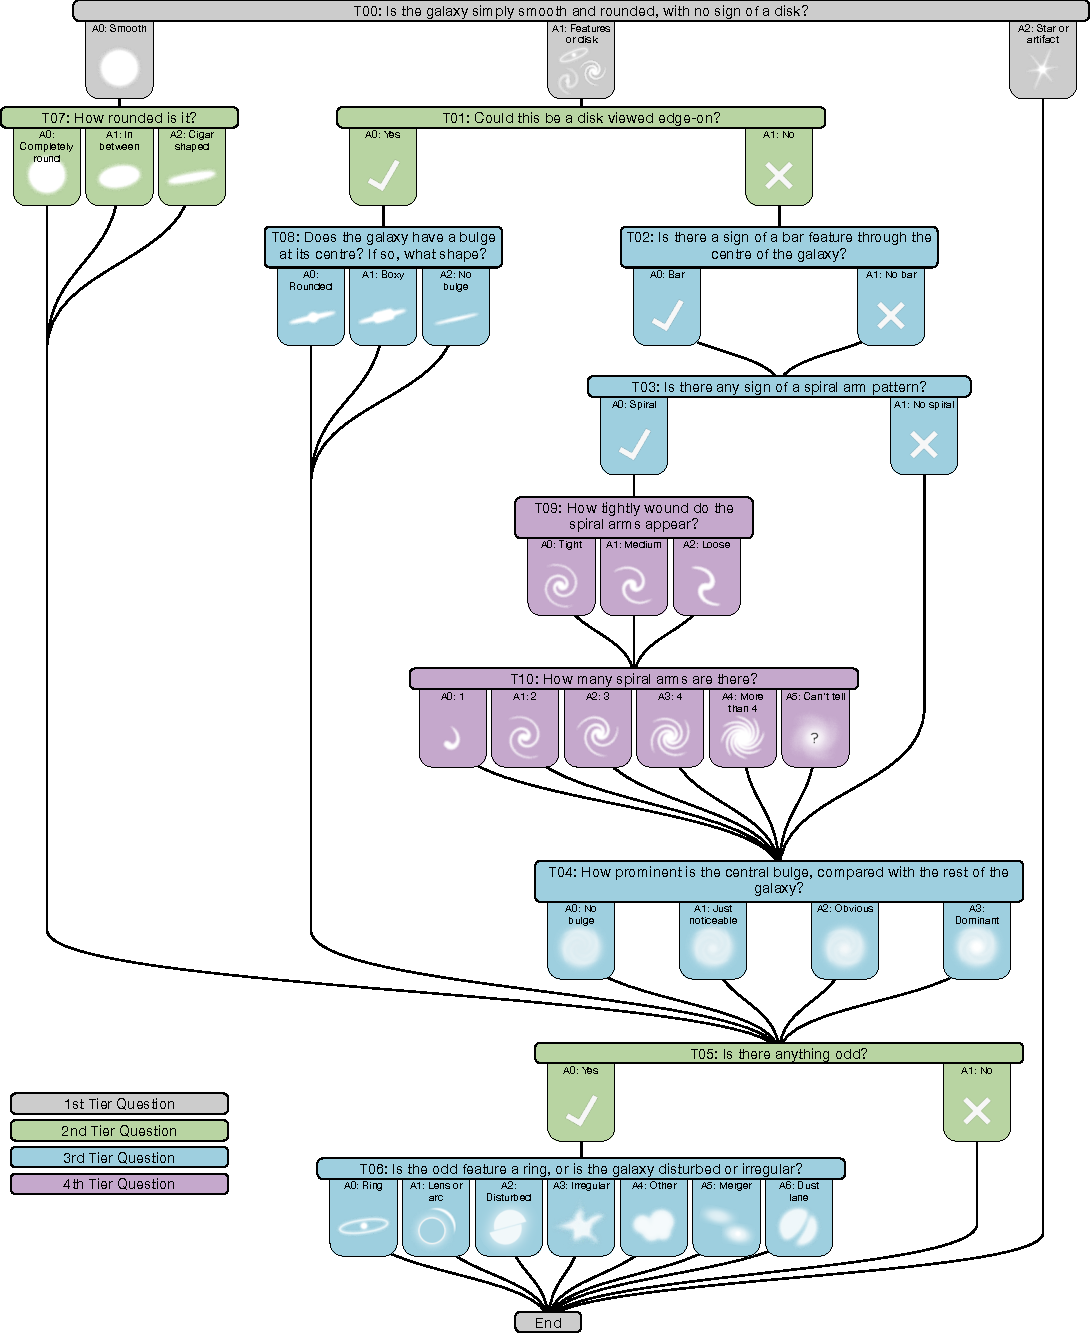
\includegraphics[width=\textwidth]{introduction/gz2_tree.pdf}}
\caption[GZ2 classification decision tree]{Flowchart of the classification tree for GZ2, beginning at the top. Tasks are colour-coded by their relative depths in the decision tree with tasks in green, blue and purple respectively one, two or three steps below branching points in the decision tree.}
\label{tree}
\end{figure}

The Galaxy Zoo 2 (GZ2) project consists of $304, 022$ images from the SDSS DR8 (a subset of those classified in Galaxy Zoo 1; GZ1) all classified by \emph{at least} 17 independent users, with the mean number of classifications standing at $\sim42$. The GZ2 sample is more robust than the GZ1 sample and provides more detailed morphological classifications, including features such as bars, the number of spiral arms and the ellipticity of smooth galaxies. It is for these reasons I use the GZ2 sample, as opposed to the GZ1, allowing for further investigation of specific galaxy classes in the future. 

\begin{figure*}
\centering{
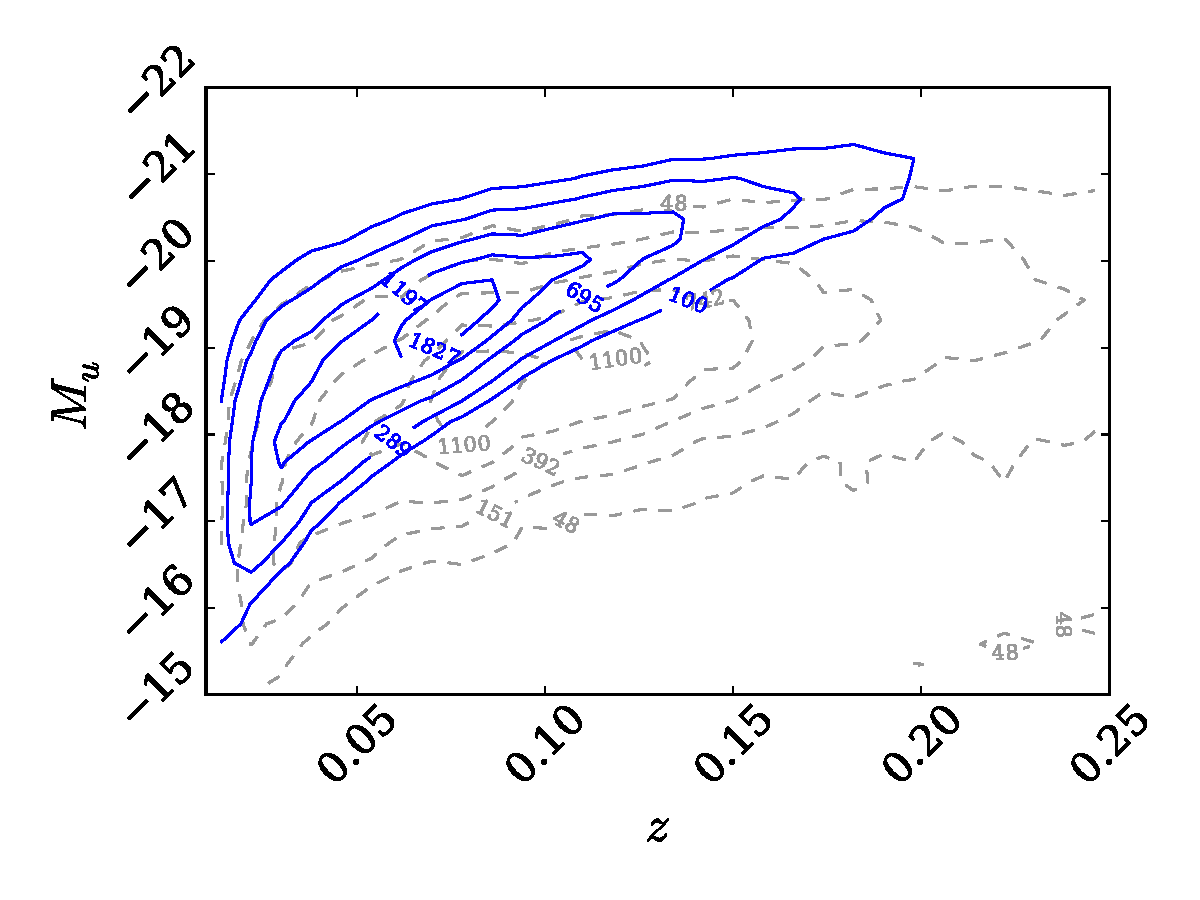
\includegraphics[width=0.8\textwidth]{introduction/mag_redshift_completeness.pdf}}
\caption[GZ2-GALEX sample completeness]{Absolute $u$-band magnitude against redshift for the whole of SDSS (grey dashed lines) in comparison to the GZ2 subsample (blue solid lines). Typical Milky Way $L_*$ galaxies with $M_u \sim -20.5$ are still included in the GZ2 subsample out to the highest redshift of $z \sim 0.25$.}
\label{complete}
\end{figure*}

\begin{figure}
\centering{
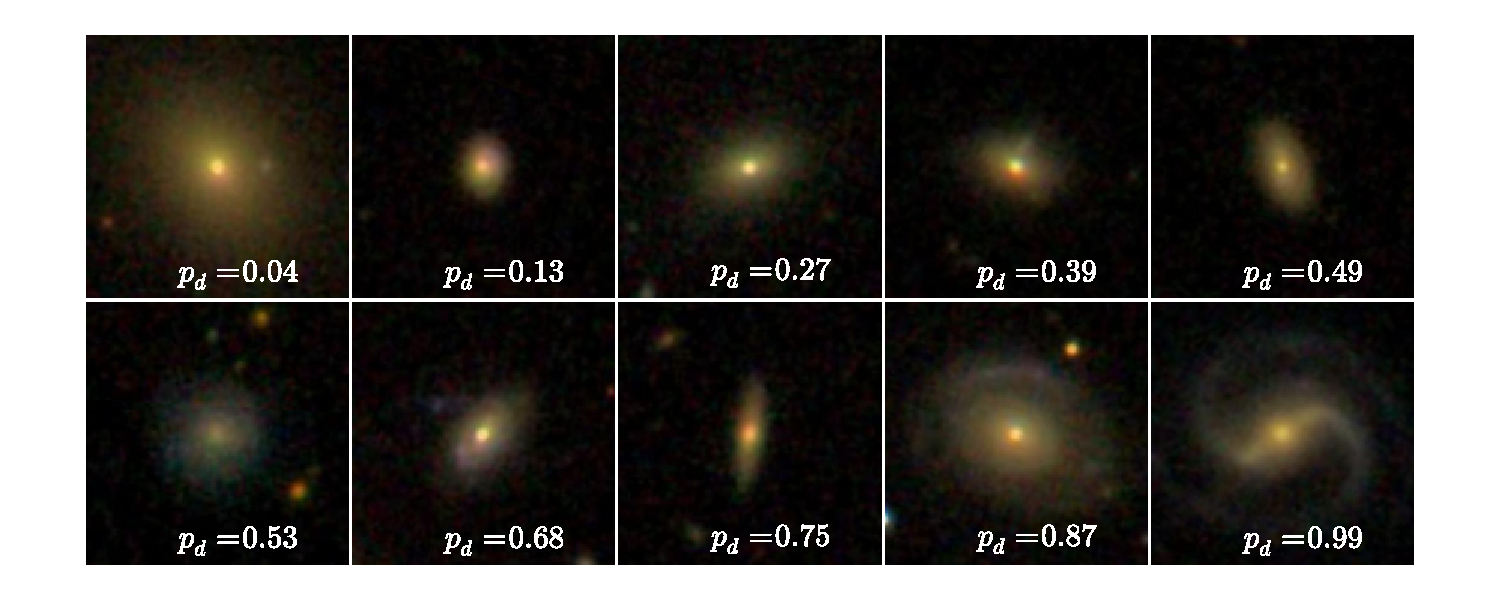
\includegraphics[width=\textwidth]{introduction/mosaic_disc_fraction_z_0-07_0-075.pdf}}
\caption[Example SDSS images with GZ2 vote fractions]{Randomly selected SDSS \emph{gri} composite images showing the continuous probabilistic nature of the Galaxy Zoo sample from a redshift range $0.070 < z < 0.075$. The debiased disc vote fraction (see \citealt{GZ2}) for each galaxy is shown. The scale for each image is $0.099~\rm{arcsec/pixel}$.}
\label{mosaic}
\end{figure}


The decision tree that users are led through whilst classifying galaxies with GZ2 is shown in Figure~\ref{tree}. The first task of GZ2 asks users to choose whether a galaxy is mostly smooth, is featured and/or has a disc or is a star/artefact. Unlike other tasks further down in the decision tree, every user who classifies a galaxy image will complete this task (others, such as whether the galaxy has a bar, is dependent on a user having first classified it as a featured galaxy). Therefore I have the most statistically robust classifications at this level.

The classifications from users produces a vote fraction for each galaxy (the debiased fractions calculated by \citet{GZ2} were used in this investigation); for example if 80 of 100 people thought a galaxy was disc shaped, whereas 20 out of 100 people thought the same galaxy was smooth in shape (i.e. elliptical), that galaxy would have vote fractions $p_{s} = 0.2$ and $p_{d} = 0.8$. In this example this galaxy would be included in the \emph{`clean'} disc sample ($p_d \geq 0.8$) according to \cite{GZ2} and would be considered a late-type galaxy. All previous Galaxy Zoo projects have incorporated extensive analysis of volunteer classifications to measure classification accuracy and bias, and compute user weightings (for a detailed description of debiasing and consistency-based user weightings, see either Section 3 of \citealt{Lintott09} or Section 3 of \citealt{GZ2}). 


The classifications are highly accurate and provide a continuous spectrum of morphological features, as shown in Figure~\ref{mosaic}, rather than a simple binary classification separating elliptical and disc galaxies. These classifications allow each galaxy to be considered as a probabilistic object with both bulge and disc components. 

\section{Defining the GZ2-GALEX main galaxy sample}\label{sec:defsample}

The only selection that was made on the GZ2 sample was to remove objects considered to be stars, artefacts or merging pairs by the users (i.e. with $p_{star/artefact} ~\geq~ 0.8$ or $p_{merger} ~\geq 0.420$; see \citealt{GZ2} Table 3 and discussion for details of this fractional limit). Further to this, I required NUV photometry from the GALEX survey, within which $\sim42\%$ of the GZ2 sample were observed, giving a total sample size of $126, 316$ galaxies. This will be referred to as the \textsc{gz2-galex} sample. 

The completeness of the \textsc{gz2-galex} sample is shown in Figure~\ref{complete} with the $u$-band absolute magnitude against redshift, compared with the SDSS data set. Typical Milky Way $L_*$ galaxies with $M_u \sim -20.5$ are still included in the GZ2 subsample out to the highest redshift of $z \sim 0.25$; however dwarf and lower mass galaxies are only detected at the lowest redshifts.

Galaxy colours were not corrected for intrinsic dust attenuation. This is of particular consequence for disc galaxies, where attenuation increases with increasing inclination. \cite{Buat05} found the median value of the attenuation in the GALEX NUV passband to be $\sim 1$ mag. Similarly \cite{masters10a} found a total extinction from face-on to edge-on spirals of 0.7 and 0.5 mag for the SDSS $u$ and $r$ passbands and show spirals with $\log(a/b) > 0.7$ have signs of significant dust attenuation. For the \textsc{gz2-galex} sample I find $?\%$ of discs (with $p_d > 0.5$) have $\log(a/b) > 0.7$, therefore we must be aware of possible biases in the results due to dust. 

I shall use the \textsc{gz2-galex} sample to probe how different quenching mechanisms cause galaxies to transition from the SFS to quiescence. 

%From the findings of \cite{masters10a} and \cite{Buat05} above, I estimate the extinction to be $u-r \sim 0.2$ mag and $NUV-u \sim 0.3$ mag, therefore the average change in the SFH parameters across a range of input colours $0 ~<~u-r~<~4$ and $-1~<~NUV-u~<~5$,  are $\Delta~t_q~=~0.985$~Gyr, $\Delta~\tau~=~1.571$~Gyr. This change therefore causes the SFH parameters derived to move towards earlier times and faster quenching rates. Results should be viewed with the caveat, particularly for higher mass, disc galaxies, that earlier values of $t_q$ and more rapid values of $\tau$ may be inferred by \textsc{starpy}. However, I note that (i) applying these average corrections across each sample population does not change our main conclusions, (ii) that results are consistent if the population of edge-on and face-on galaxies are compared (see Figure~\ref{dustsplit} and (iii) that results do not change if only face-on galaxies are used in the investigation, strongly suggesting that internal galactic extinction does not systematically bias our results.
